\chapter{Augmented Reality Library for the Web (tracking.js)} % (fold)
\label{cha:ar_library_for_the_web}

\section{Introduction} % (fold)
\label{sec:ar_library_for_the_web:introduction}

The desktop platform is the target environment most commonly addressed when developing Augmented Reality (AR) systems. However, depending on the requirements of an AR application, the use of different execution platforms may be necessary. If the system has to be published to several users, the web platform shows to be more adequate, where the application is executed through the Internet in a web browser \cite{Pablo2013}.
The use of markerless tracking, which is based on natural features of the scene, has also been gaining more space on web targeted AR applications for advertising. The media used in this kind of application needs to be as appealing as possible in order to catch consumers’ attention. Markerless tracking satisfies this requirement, since the idea of having a real scene augmented with virtual objects without any artificial elements such as markers added to the environment is very attractive \cite{Pablo2013}. In addition, the product being advertised can be tracked and augmented with virtual elements \cite{Pablo2013}.
Browsers are evolving very fast when compared to the the previous decade \cite{Hickson2013}. JavaScript language \cite{International2009,MDN2013} wasn't prepared to handle typed data structures \cite{TypedArray2013} able to manipulate raw binary data safely \cite{Canvas2013}, all the computational complexity required by AR algorithms was too much for that growing environment. Browsers weren't able to capture audio and video \cite{MediaCapture2013,WebRTC2013} natively, without plugin installation \cite{Flash2013}, an essential feature for AR applications. This reality has changed, this involves the use of several modern browser specifications \cite{Hickson2013,WC2006} as well as implementation of different computer vision algorithms and techniques into the browser environment taking advantage of all those modern APIs \cite{Hickson2013,WC2006}.

In this context, this thesis aims to present the implementation and evaluation of some solutions regarding markerless tracking for web targeted AR. Some optimizations are discussed and implemented on this work in order to achieve good results when compared with similar implementations in compiled languages.

% section introduction (end)

\section{Related Work} % (fold)
\label{sec:ar_library_for_the_web:related_work}

There are not many web based RA solutions available and registered in the literature. The ones available are mainly focused on fiducial markers \cite{Cho1998}, such as FLARToolKit \cite{Yan2011} and JSARToolkit \cite{JSARToolkit2011}, they both are ports of ARToolKit \cite{Hirokazu2002}. ARToolKit is a desktop library which is useful to make vision-based Augmented Reality applications \cite{Hirokazu2002}. The Metaio company developed Unifeye Viewer \cite{Metaio2009}, a proprietary plug-in for Flash \cite{Flash2013} that allows the utilization of markerless AR applications on the web. In order to run Flash \cite{Flash2013} based applications, the instalation of its plugin is required. Third-party plugins, such as Flash \cite{Flash2013}, are in decadency on modern and mobile web browsers, instead JavaScript \cite{International2009} based solutions are preffered, since they can run in any modern browser without required any user effort of installing external software. Some smart-phones doesn't even support Flash \cite{Flash2013} plugin into their browsers, \eg\ Safari for mobile \cite{Safari2013} is one example of a mobile browser that have banned Flash \cite{Flash2013}.

\begin{enumerate}
    \item FLARToolKit: is a port of the well-known ARToolKit \cite{Hirokazu2002} marker tracking library to ActionScript \cite{Flash2013}, which is the language utilized in the development of Flash \cite{Flash2013} applications for the web. This was the first initiative towards AR solutions for the web \cite{Pablo2013}. Using FLARToolKit, is possible to develop AR applications that runs on client's browser. A marker based AR example for the web developed for a marketing campaing of General Electric's company using FLARToolKit is shown on Figure \ref{figure:flartoolkit}.

    \begin{figure}[!htb]
      \centering
      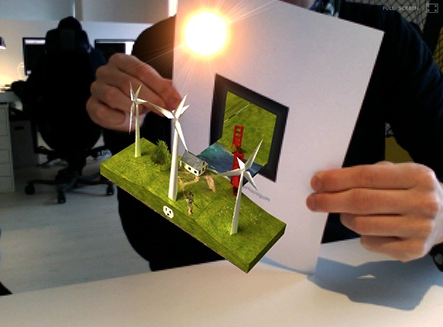
\includegraphics[width=240pt]{chapters/computer_vision_library_for_the_web/flartoolkit.png}
      \caption{Marker based AR for the web using FLARToolKit}
      \label{figure:flartoolkit}
    \end{figure}

    \item JSARToolkit: is a JavaScript \cite{International2009} port of FLARToolKit \cite{Yan2011}, operating on canvas images \cite{Canvas2013} and
video element \cite{Hickson2013} contents, provides another marker tracking library. This was the first, open-source, JavaScript \cite{International2009} based, AR solution available for the web. A marker based AR example for the web using JSARToolKit is shown on Figure \ref{figure:jsartoolkit}.

    \begin{figure}[!htb]
      \centering
      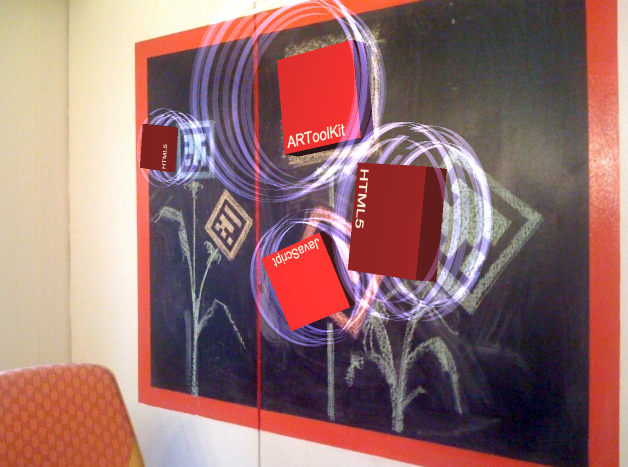
\includegraphics[width=240pt]{chapters/computer_vision_library_for_the_web/jsartoolkit.png}
      \caption{Marker based AR for the web using JSARToolKit}
      \label{figure:jsartoolkit}
    \end{figure}

    \item Unifeye Viewer: from Metaio company, offers a robust markerless tracking solution. Unifeye \cite{Metaio2009} also depends on Flash \cite{Flash2013} plugin in order to run on web browsers. A similar example of General Electric's marker based, previously shown on Figure \ref{figure:flartoolkit}, is a markerless based using Unifeye Eye \cite{Metaio2009} shown on Figure \ref{figure:unifeyeviewer}. Note that the 3D image is projected over a magazine cover instead of a fiducial marker \cite{Cho1998}.

    \begin{figure}[!htb]
      \centering
      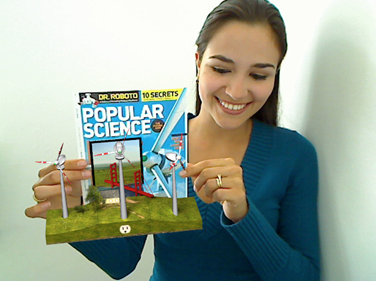
\includegraphics[width=240pt]{chapters/computer_vision_library_for_the_web/unifeyeviewer.png}
      \caption{Marker based AR for the web using JSARToolKit}
      \label{figure:unifeyeviewer}
    \end{figure}
\end{enumerate}

% section related_work (end)

\section{Marker-less Tracking Algorithm (Keypoints)} % (fold)
\label{sec:ar_library_for_the_web:marker_less_tracking_algorithm}

Lorem ipsum dolor sit amet, consectetur adipisicing elit.

% section marker_less_tracking_algorithm (end)

\section{Interest Point Detection} % (fold)
\label{sec:ar_library_for_the_web:interest_point_detection}

This technique rely on matching individual features across images and are therefore easy to robustify against partial occlusions or matching errors. Illumination invariance is also simple to achieve. Feature Points detection is used as the first step of many vision tasks such as tracking, localization, image matching and recognition. In this article we call ``feature'' or ``keypoint'' to refer to a point of interest in two dimensions.

The algorithms perform a simple loo and for each frame, the object features are matched by localizing feature templates in search windows around hypothesized locations \cite{Lepetit2005}. The method to extract feature points suggested in Features from Accelerated Segment Test (FAST) \cite{Rosten2010}. FAST hypothesizes the matches using corner detection. A large number of corner detectors exist in the literature. However, we have a strong interest in realtime frame rate applications which computational resources are required requisites. The approach proposed by FAST allows the detector to produce a suite of high-speed detectors which we currently use for real-time tracking and AR label placement \cite{Calonder2010}. In particular, it is still true that when processing live video streams at full frame rate, existing feature detectors leave little if any time for further processing, even despite the consequences of Moore’s Law \cite{Rosten2010}.

To show that speed can been obtained without necessarily sacrificing the quality of the feature detector, in Chapter \ref{cha:evaluation}, we compare our detector, to a variety of well-known detectors. A number of the detectors described below compute a corner response, (1) Edge based corner detectors, corresponds to the boundary between two regions; (2) Greylevel derivative based detectors, the assumption that corners exist along edges is an inadequate model for patches of texture and point like features, and is difficult to use at junctions. Therefore a large number of detectors operate directly on greylevel images without requiring edge detection; and (3) Direct greylevel detectors, Another major class of corner detectors work by examining a small patch of an image to see if it ``looks'' like a corner \cite{Rosten2010}.

The thesis choice was (3) Direct greylevel detectors. It works by testing a small patch of an image to see if it could be a corner. The detector is evaluated using a circle surrounding the candidate pixel, the test is based on whether the concentric contiguous arcs around the pixel are significantly different from the central pixel $p$ \cite{Rosten2010}. To classify $p$ as a corner should exists a set of $n$ contiguous pixels in the circle which are all brighter than the intensity of the candidate pixel $I_{p} + t$ (threshold), or all darker than $I_{p} - t$ \cite{Rosten2010}.

The number of contiguous tested pixels could vary accordingly \cite{Rosten2010}, being more common to be FAST-$12$ or FAST-$9$. Empirically, FAST-$9$ showed to have a good repeatability and a better efficiency on the web. The repeatability of found feature points is also important because determines whether the technique is useful in a real-world application.

This detector in itself exhibits high performance, but there are several weaknesses: (1) This high-speed test does not reject as many candidates; (2) The efficiency of the detector will depend on the ordering of the questions and the distribution of corner appearances; and (3) Multiple features are detected adjacent to one another \cite{Rosten2010}.

On Figure \ref{figure:fast}, the highlighted squares are the pixels used in the corner detection. The pixel at $p$ is the central pixel. The arc is indicating that the dashed line passes through FAST-$n$, let $n$ be $9$ or $12$ contiguous pixels which are brighter or darker than $p$ \cite{Rosten2010}.

\begin{figure}[!htb]
  \centering
  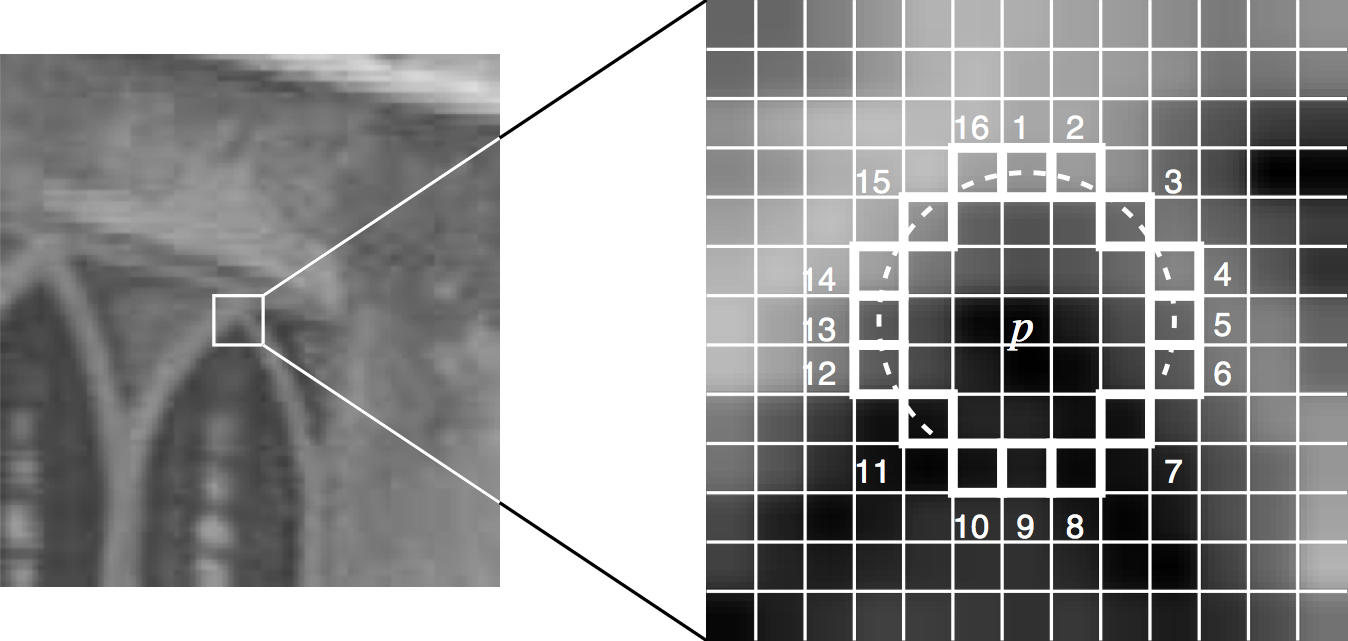
\includegraphics[width=\linewidth]{chapters/computer_vision_library_for_the_web/fast.png}
  \caption{Point segment test corner detection in an image patch \cite{Glass2013}}
  \label{figure:fast}
\end{figure}

% section interest_point_detection (end)

\section{Interest Point Matching} % (fold)
\label{sec:ar_library_for_the_web:interest_point_matching}

To estimate motion, one can then match sets of interest points \{$m_{i}$\} and \{$m'_{j}$\} extracted from two images taken from similar, and often successive, viewpoints. A classical procedure \cite{Calonder2010} runs as follows. For each point \{$m_{i}$\} in the first image, search in a region of the second image around location \{$m_{i}$\} for point \{$m'_{j}$\}. The search is based on the similarity of the local image windows centered on the points, which strongly characterizes the points when the images are sufficiently close \cite{Lepetit2005}.

The feature matching used in the case studies performed in this work search for correspondent points in the current frame. Only points that are highly descriptive invariant features, called keypoints, are tested. Those keypoints were detected using FAST \cite{Rosten2010} in Section \ref{sec:ar_library_for_the_web:interest_point_detection}.

Since web and handled devices have limited computational power having local descriptors that are fast to compute, to match and being memory efficient are important aspects, therefore an efficient method Binary Robust Independent Elementary Features (BRIEF) \cite{Calonder2010} was used.

Distance metric is critical to the performance of intrusion detection systems. Thus using binary strings reduces the size of the descriptor and provides an interesting data structure that is fast to operate with whose similarity can be measured by the Hamming distance which, on desktop implementations, the computation time could be driven almost to zero using the POPCNT instruction from SSE4.2 \cite{Intel2007}. Only the latest Intel Core i7 CPUs support this instruction.

The Hamming distance is an important step on interest point matching, it provides a fast and memory-efficient way to calculate distance between binary strings. Given two image patches $x$ and $y$, denote their binary descriptors as $b(x) \in \{0,1\}^n$ and $b(y) \in \{0,1\}^n$ respectively. Then their Hamming distance is computed by:

$$Ham(x, y)=\sum_{i=1}^{n}b_i(x)\otimes b_i(y)$$

In which $n$ is the dimension of binary descriptor and stands for bitwise XOR operation. According to the definition of Hamming distance, all the elements of a binary descriptor contribute equally to the distance. From the hamming distance, the Hamming weight can be calculated. It is used to find the best feature point match. Here, is generalized the Hamming distance to the weighted Hamming:

$$WHam(x, y)=\sum_{i=1}^{n}w_i(b_i(x)\otimes b_i(y))$$

Where $w_i$ is the weight of the $i$th element. The goal is to learn $w_i,i=1,2\cdots,n$ for the binary descriptor (BRIEF) based on a set of feature points. By assigning different weights to binary codes, what we expect is to obtain a distance space in which the distances of matching patches are less than those of non-matching patches.

To generate the binary string for each key-point found in the smoothed frame, the individual bits are obtained by comparing the intensities of pairs of points along the kernel window centered on each key-point without requiring a training phase. Empirically, this technique shows that 256 bits or even 128 bits, often suffice to obtain very good matching results and the best spatial arrangement of the tested (\textbf{x}, \textbf{y})-pairs of points have better results when selected based on an isotropic Gaussian distribution, which could be simply replaced by a random function due to its random characteristics.

To generate the binary strings is defined test $\tau$ on patch \textbf{p} of size \textbf{S $\times$ S} as

$$\tau(\textbf{p}; x, y) :=
\begin{cases}
  1 &\mbox{if}\quad \textbf{p(x)} < \textbf{p(y)},\\
  0 &\mbox{otherwise}
\end{cases}$$

where \textbf{p(x)} is the pixel intensity. The set of binary tests is defined by the $n_{d}$ (\textbf{x}, \textbf{y})-location pairs uniquely chosen during the initialization. The $n_{d}$-dimensional bit-string is our BRIEF descriptor for each key-point

$$f_{n_{d}}(\textbf{p}) := \sum_{1 \le i \le n_{d}} 2^{i-1} \tau(\textbf{p}; x, y).$$

In \cite{Calonder2010}, $n_{d}=$ 128, 256, and 512 were used in the tests and any of those values yield good compromises between speed, storage efficiency, and recognition rate. The number of bytes required to store the descriptor can be calculated by $k = n_{d}/8$, proving that BRIEF is also a memory-efficient method. Detailed results can be found in Chapter \ref{cha:evaluation}.

% section interest_point_matching (end)

\section{Pose Estimation} % (fold)
\label{sec:ar_library_for_the_web:pose_estimation}

Lorem ipsum dolor sit amet, consectetur adipisicing elit.

% section pose_estimation (end)

% chapter ar_library_for_the_web (end)